\documentclass[a4paper,10pt]{article}

\pagestyle{empty}


%%%%%%%%%%%%%%%%%%%%%%%%%%%%%%% Paquetes %%%%%%%%%%%%%%%%%%%%%%%%%%%%%%%%%%%

\usepackage[ansinew]{inputenc}
\usepackage[spanish]{babel}
\usepackage[mathcal]{euscript}
\usepackage{amsmath,amsfonts,amssymb,theorem,latexsym,mathrsfs, %hyperref,
            epsfig, multicol,anysize,graphicx,enumitem,mdwlist}
\usepackage{graphicx}  
\usepackage{ragged2e}  
\usepackage{float}        


%%%%%%%%%%%%%%%%%%%%%%%%%%%%%%%%%%%%%%%%%%%%%%%%%%%%%%%%%%%%%%%%%%%%%%%%%%%%


%%%%%%%%%%%%%%%%%%%%%%%%%%%%%%% M�rgenes %%%%%%%%%%%%%%%%%%%%%%%%%%%%%%%%%%%

\marginsize{2cm}{1.5cm}{1cm}{2cm}

%\marginsize{izquierdo}{derecho}{arriba}{abajo}

%%%%%%%%%%%%%%%%%%%%%%%%%%%%%%%%%%%%%%%%%%%%%%%%%%%%%%%%%%%%%%%%%%%%%%%%%%%%


%%%%%%%%%%%%%%%%%%%%%%%%%%%%% Definiciones %%%%%%%%%%%%%%%%%%%%%%%%%%%%%%%%%

\def\r{\mathbb{R}}
\def\n{\mathbb{N}}
\def\q{\mathbb{Q}}
\def\c{\mathbb{C}}
\def\z{\mathbb{Z}}

\def\sen{\mathop{\mbox{\normalfont sen}}\nolimits}
\def\intt{\mathop{\mbox{\normalfont int}}\nolimits}
\def\diag{\mathop{\mbox{\normalfont diag}}\nolimits}
\def\arcsen{\mathop{\mbox{\normalfont arcsen}}\nolimits}
\def\ln{\mathop{\mbox{\normalfont ln}}\nolimits}
\def\tr{\mathop{\mbox{\normalfont tr}}\nolimits}

%%%%%%%%%%%%%%%%%%%%%%%%%%%%%%%%%%%%%%%%%%%%%%%%%%%%%%%%%%%%%%%%%%%%%%%%%%%%

\begin{document}

%%%%%%%%%%%%%%%%%%%%%%%%%%%% Encabezado %%%%%%%%%%%%%%%%%%%%%%%%%%%%%%%%%%%%

\begin{minipage}{0.12\linewidth}

\includegraphics[width=15mm]{escudo.jpg}
\end{minipage}
\begin{minipage}{0.78\linewidth}
\centerline{UNIVERSIDAD DE ANTIOQUIA}
\centerline{Facultad de Ciencias Exactas y Naturales}
\centerline{Instituto de Matem�ticas}
\centerline{Series de Tiempo II}
\centerline{Taller $\#$ 2}
\end{minipage}

\vspace{3mm}

\leftline{Profesor: Duv�n Cata�o}


\vspace{8mm}


\begin{enumerate}

\item A time series was generated by first drawing the white noise series wt from a normal distribution with mean zero and variance one. The observed series $x_t$ was generated from

$$x_t=w_t-\theta w_{t-1}, \ \ \ \ t=0,\pm1,\pm2,\ldots,$$

where $\theta$ is a parameter.

\begin{enumerate}
\item Derive the theoretical mean value and autocovariance functions for the series $x_t$ and $w_t$ . Are the series $x_t$ and $w_t$ stationary? Give your reasons.

\item Give a formula for the power spectrum of $x_t$ , expressed in terms of $\theta$ and $w$.
\end{enumerate}

\bigskip

\item  In applications, we will often observe series containing a signal that has been delayed by some unknown time $D$, i.e.,

$$x_t = s_t + As_{t-D} + n_t,$$

where $s_t$ and $n_t$  are stationary and independent with zero means and spectral densities $f_s(w)$ and $f_n(w)$, respectively. The delayed signal is multiplied by some unknown constant $A$. Show that

$$f_x(w)=[1+A^2 +2Acos(2\pi wD)]f_s(w)+ f_n(w).$$

\bigskip

\item Consider $y_t=h_tx_t$, for $t=0,1,\ldots,T-1$, and using the modified DFT:

$$Y(v_k)=c^{-1/2}\sum_{t=0}^{T-1}x_th_te^{-2\pi iv_kt},$$

with $c=\sum_{t=0}^{T-1}h_t^2$. 

Prove that 
$$\mathbb{E}|Y(v_k)|^2=\int_{-1/2}^{1/2}|H(v_k-v)|^2f_x(v)dv,$$

with $H(v)=c^{-1/2}\sum_{t=0}^{T-1}h_te^{-2\pi ivt}.$  

\bigskip


\item Suppose $x_t$ and $y_t$ are stationary zero-mean time series with $x_t$ independent of $y_s$ for all $s$ and $t$. Consider the product series

$$z_t =x_ty_t.$$ 

Prove the spectral density for $z_t$ can be written as
$$f_z(w) =\int_{-1/2}^{1/2}f_x(w - v)f_y(v)dv.$$

\bigskip

\item With sample size to $n = 128$,  generate and plot the time series as
$$x_{t1} = 2\cos(2\pi 0.06t)+3\sin(2\pi 0.06t)$$
$$x_{t2} = 4\cos(2\pi 0.10t)+5\sin(2\pi 0.10t)$$
$$x_{t3} = 6\cos(2\pi 0.40t)+7\sin(2\pi 0.40t)$$
 $$x_t =x_{t1}+x_{t2}+x_{t3}.$$
 
 \begin{enumerate}
 
 \item Compute and plot the periodogram of the series, $x_t$ , generated above and comment.
 
\item Repeat the analyses adding noise to $x_t$ ; that is

$$x_t =x_{t1}+x_{t2}+x_{t3}+w_t$$

where $w_t \sim iid \ \mathcal{N}(0, 25)$. That is, you should simulate and plot the data, and then plot the periodogram of $x_t$ and comment.
\end{enumerate}

\bigskip

\item Figure 4.22 shows the biyearly smoothed (12-month moving average) number of sunspots from June 1749 to December 1978 with $n = 459$ points that were taken twice per year; the data are contained in \emph{sunspotz}. With Example 4.13 as a guide, perform a periodogram analysis identifying the predominant periods and obtaining confidence intervals for the identified periods. Interpret your findings.

\item  The levels of salt concentration known to have occurred over rows, corresponding to the average temperature levels for the soil science data considered in Figs. 1.18 and 1.19, are in \emph{salt} and \emph{saltemp}. Plot the series and then identify the dominant frequencies by performing separate spectral analyses on the two series. Include confidence intervals for the dominant frequencies and interpret your findings.
 
 \bigskip
 
 \item Let $\{w_t;t=0,1,\ldots \}$ be a white noise process with variance 
 $\sigma_w^2$ and let $|\phi|<1$ be a constant. Consider the process $x_0 = w_0$, and
$$x_t=\phi x_{t-1} + w_t, \ \ t=1,2,\ldots.$$ 

We might use this method to simulate an AR$(1)$ process from simulated white noise.
\begin{enumerate}
\item Show that $x_t=\sum_{j=0}^t\phi^jw_{t-j}$ for any $t=0,1,\ldots.$
\item  Find the $\mathbb{E}(x_t ).$
\item  Show that, for $t = 0, 1, \ldots,$

$$\mathbb{V}ar(x_t)=\frac{\sigma_w^2}{1-\phi^2}({1-\phi^{2(t+1)})$$

\item  Show that, for $h \geq 0$,
$$\mathbb{C}ov(x_{t+h},x_t)=\phi^h\mathbb{V}ar(x_t)$$
\item  Is $x_t$ stationary?
\item  Argue that, as $t\rightarrow\infty$, the process becomes stationary, so in a sense, $x_t$ is ''asymptotically stationary."
\item  Comment on how you could use these results to simulate $n$ observations of a stationary Gaussian AR$(1)$ model from simulated iid $N(0,1)$ values.
\item  Now suppose $x_0 = w_0/\sqrt{1 - \phi^2}.$ Is this process stationary? 
Hint: Show $\mathbb{V}ar(x_t)$ is constant.
\end{enumerate}

\bigskip

\item Suppose we would like to predict a single stationary series $x_t$ with zero mean and autocorrelation function $\gamma(h)$ at some time in the future, say, $t + l,$ for $l > 0.$
\begin{enumerate}
\item If we predict using only $x_t$ and some scale multiplier $A$, show that the mean-square prediction error 

$$MSE(A) = \mathbb{E}[(x_{t+l}-Ax_t)^2]$$

is minimized by the value
$$ A = \rho(l).$$

\item Show that the minimum mean-square prediction error is 
$$MSE(A) = \gamma(0)[1 - \rho^2(l)].$$

\item Show that if $x_{t+l} =Ax_t,$ then $\rho(l)=1$ if $A>0$, and $\rho(l)=-1$ if $A<0.$
\end{enumerate}

\bigskip

\item For the process $y_t=\sum_{j=-\infty}^{\infty}a_jx_{t-j}$, with $\sum_{j=-\infty}^{\infty}|a_j|<\infty,$ if $x_t$ has spectrum $f_x(w)$, then the spectrum of the filtered output, $y_t$ , say $f_y(w)$, is related to the spectrum of the input $x_t$ by
$$f_y(w)=|A(w)|^2f_x(w)$$
where the frequency response function $A(w)=\sum_{j=-\infty}^{\infty}a_je^{-2\pi iwj}.$

\bigskip

\item Suponga que los residuos $\hat{a}_t$ del modelo $(1-B)Z_t=(1+0,6B)a_t,$ ajustado de una serie de 80 observaciones, proporcionan las siguientes autocorrelaciones:

\begin{table}[htdp]
\begin{center}\begin{tabular}{c|cccccccccc}
$h$ & 1 & 2 & 3 & 4 & 5 & 6 & 7 & 8 & 9 & 10  \\
\hline
$\rho_{\hat{a}}(h)$ & 0.39 & 0.20 & 0.09 & 0,04 & 0,09 & -0.13 & -0.05 & 0.06 & 0.11 & -0.02 
\end{tabular} 
\end{center}
\label{defaulttable}
\end{table} 
\begin{enumerate}
\item Analice la adecuaci{\'o}n del modelo ajustado y si existe alguna indicaci{\'o}n de falta de ajustamiento del modelo. Si esto ocurre, sugiera un modelo modificado y pru{\'e}belo. 

\item Calcular la densidad espectral del modelo encontrado en el numeral anterior. Haga las suposiciones necesarias para garantizar la existencia del mismo.
\end{enumerate}

\bigskip

\item Probar que $$\gamma(h)=\left\{\begin{array}{l}
1, \ \ h=0 \\
\rho,  \ \  h=\pm1 \\
0,  \ \  o.c\end{array}\right.$$
es una funci{\'o}n de autocovarianza si y s{\'o}lo si $|\rho|<1/2.$

\bigskip

\item Obtener el espectro del proceso cuya funci{\'o}n de autocovarianza es dada por $$\gamma(t)=Me^{-\alpha|\tau|}cos(\beta t),$$

donde $M>0,$ $\alpha>0$, $\beta>0$ y $\tau\in\mathbb{R}.$

\bigskip

\item Sea $Z_t=a_{t}+ca_{t-1}+ca_{t-2}+\ldots+ca_1$, para $t>0,$ donde $c\in\mathbb{R}$ y $a_t\sim RB(0, \sigma_a^2).$
\begin{enumerate}
 \item Calcular la media y autocovarianza de $Z_t$. ?`Ella es estacionaria? Justifique.
 \item Calcular la media y autocovarianza de $(1-B)Z_t$. ?`Ella es estacionaria? Justifique.
\item En caso de estacionaridad en alguno de los items anteriores, calcular el espectro.
\end{enumerate}

\bigskip

\item Una serie de 400 observaciones present{\'o} los siguientes resultados:

\begin{table}[htdp]
\begin{center}\begin{tabular}{c|ccccccc}
$h$ & 1 & 2 & 3 & 4 & 5 & 6 & 7   \\
\hline
$\phi_{hh}$ & 0.8 & -0.5 & 0.07 & -0,02 & -0,01 & 0.05 & 0.04 
\end{tabular} 
\end{center}
\label{defaulttable}
\end{table} 

con $\bar{Z_t}=8$ y $\mu_o=9.$

\begin{enumerate}
\item Explique por que podemos ajustar a la series un modelo AR$(2).$
\item Obtenga las estimativas $\hat{\phi_1}$ y $\hat{\phi_2}$ del modelo AR$(2)$ utilizando las ecuaciones de Yule-Walker.
\item Verifique el modelo ajustado satisface las condiciones de estacionaridad.
\item Usando $\hat{\phi_1}$ y $\hat{\phi_2}$ como verdaderos, describa el comportamiento general de la ACF de ese proceso. 
\end{enumerate}


\end{enumerate}

\end{document}


% \begin{figure}[H]
%  \centering
%  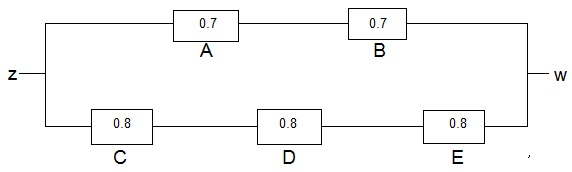
\includegraphics[width=.50\textwidth]{tab3}
% \end{figure}